\chapter{Bernapas}\label{ch:g4:breathing}

Tahanlah napasmu lalu mulailah menghitung. Jauh sebelum satu menit,
dadamu menuntut, makin lama makin mendesak, untuk bergerak lagi. Kamu
dapat melewatkan satu santapan, \omterm{prop:g1:healthy-habits:needs}{tidur} dapat menunggu sampai malam ---
tetapi udara dibutuhkan \emph{sekarang}, sepanjang waktu, kira-kira
lima belas kali semenit. Apa yang begitu mendesak di dalam satu tarikan
udara?

\section{Gerakan bernapas}

\begin{definition}[Menarik dan mengembuskan napas]\label{def:g4:breathing:movements}
Yang disebut \emph{pernapasan}\index{pernapasan} adalah pergantian
tanpa henti antara dua gerakan:
\begin{itemize}
  \item \emph{menarik napas} (inspirasi)\index{menarik napas}: dadanya
        mengembang dan udara mengalir masuk lewat hidung atau mulut;
  \item \emph{mengembuskan napas} (ekspirasi)\index{mengembuskan napas}:
        dadanya mengendur dan udara mengalir keluar kembali.
\end{itemize}
Ketika beristirahat, pasangan itu berulang kira-kira $15$ kali semenit
--- lebih cepat pada bayi, lebih cepat ketika berusaha --- tanpa kamu
pernah perlu memikirkannya.
\end{definition}

\begin{example}[Mengamati gerakannya]\label{ex:g4:breathing:watch}
Tempelkan telapak tangan pada \omterm{def:g3:bones-and-muscles:skeleton}{tulang} rusukmu: ketika \omterm{def:g4:breathing:movements}{menarik napas},
sangkar rusuknya naik dan melebar di bawah telapakmu; ketika
\omterm{def:g4:breathing:movements}{mengembuskan napas}, ia turun kembali. Sisi tubuh seekor kucing
yang tertidur memperlihatkan naik-turun yang sama. Gerakannya tidak pernah
berhenti --- terjaga, tertidur, dari tangis pertama sampai hari
terakhir.
\end{example}

\section{Ke mana udaranya pergi}

\begin{definition}[Organ pernapasan]\label{def:g4:breathing:organs}
Udara yang ditarik masuk mengembara lewat hidung (atau mulut), turun
melalui \emph{batang tenggorok}\index{batang tenggorok} --- pipa
bercincin yang kokoh, yang dapat kamu rasakan di bagian depan lehermu
--- yang lalu bercabang dua, satu ke tiap \emph{paru-paru}\index{paru-paru}.
Paru-parunya, dua organ mirip spons yang mengisi sangkar rusuk (di
balik \omterm{def:g3:bones-and-muscles:skeleton}{tulang rusuk} pada \cref{def:g3:bones-and-muscles:skeleton}),
berakhir pada jutaan kantong udara yang mungil, masing-masing
terbungkus pembuluh \omterm{prop:g4:journey-of-food:absorb}{darah} yang halus.
\end{definition}

\begin{omfigure}
\begin{tikzpicture}
  \node[anchor=south west, inner sep=0] (img) at (0,0)
    {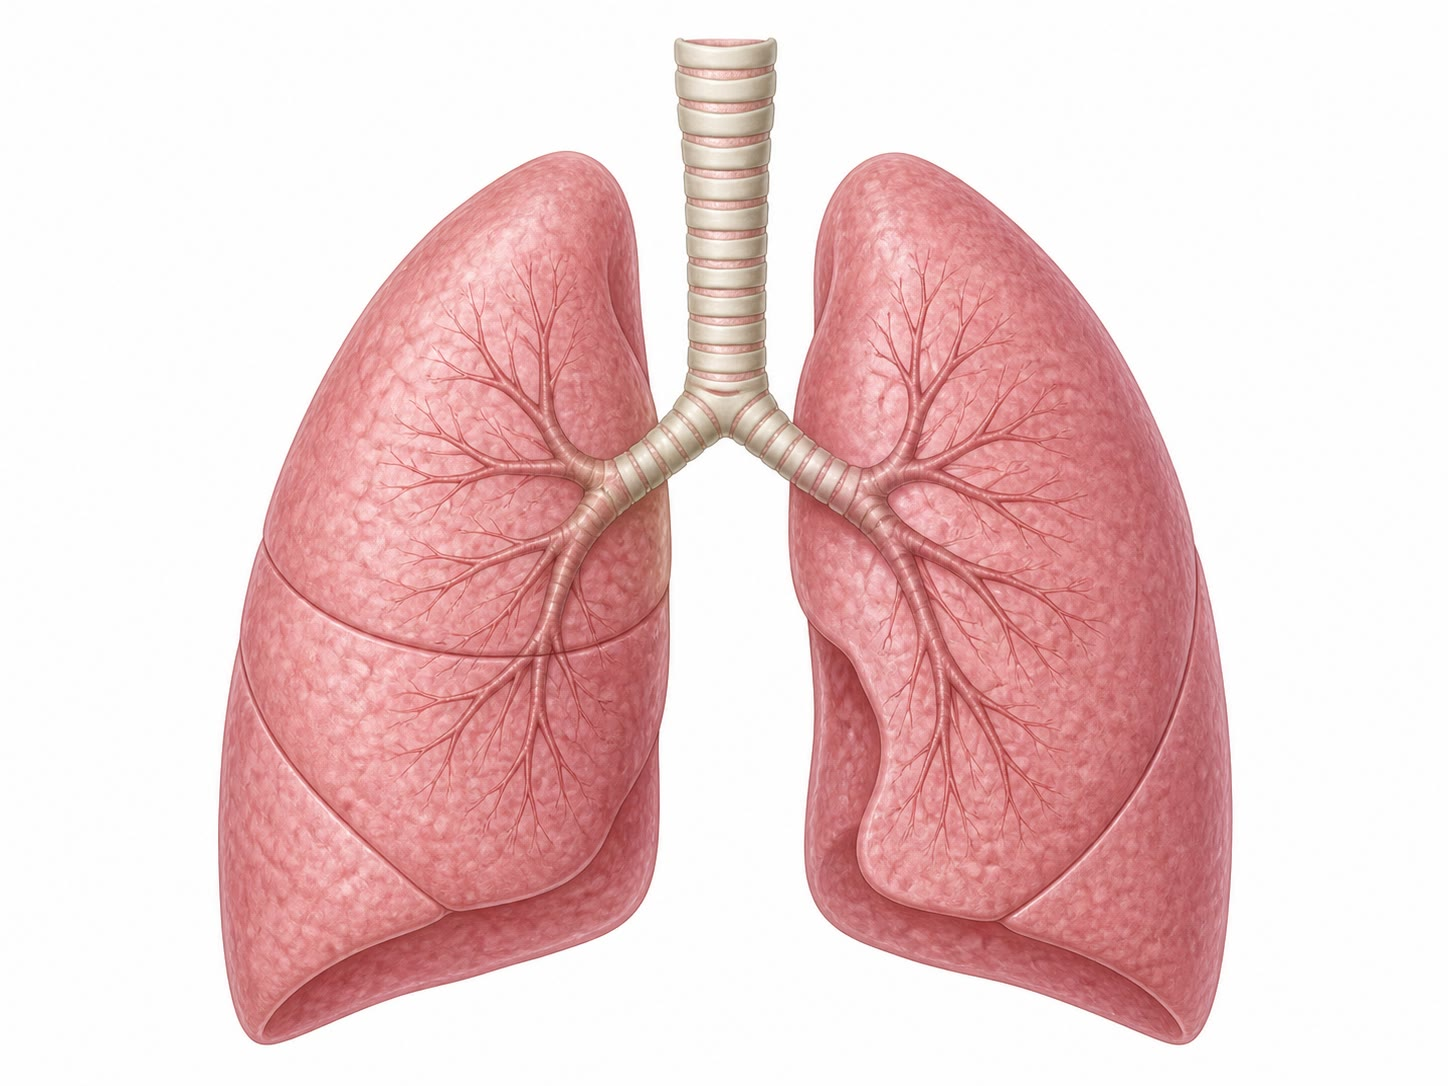
\includegraphics[width=0.58\linewidth]{images/book1/ai/fig-lungs.jpg}};
  \begin{scope}[x={(img.south east)}, y={(img.north west)},
      every node/.style={font=\small}]
    \draw[omDef, thick] (0.53,0.88) -- (0.74,0.93) node[right] {batang tenggorok};
    \draw[omDef, thick] (0.585,0.61) -- (1.03,0.64)
      node[right, align=left] {kedua\\ cabangnya};
    \draw[omDef, thick] (0.28,0.28) -- (0.11,0.13)
      node[below] {paru-paru};
  \end{scope}
\end{tikzpicture}

{\small Jalan sebuah tarikan napas: \omterm{def:g4:breathing:organs}{batang tenggorok}, dua cabang, dua
\omterm{def:g4:breathing:organs}{paru-paru} --- dan, pada ujung terhalus cabangnya, jutaan kantong udara
mungil yang terbungkus pembuluh \omterm{prop:g4:journey-of-food:absorb}{darah} halus, jauh terlalu kecil untuk
terlihat pada skala ini.}
\end{omfigure}

\begin{remark}[Berspons dengan sengaja]\label{rem:g4:breathing:sponge}
Jutaan kantong alih-alih dua kantung sederhana: itu kiat \omterm{def:g4:journey-of-food:tract}{usus halus}
sekali lagi (\cref{rem:g4:journey-of-food:surface}). Semua dinding
kantong itu menjumlah menjadi permukaan pertemuan yang amat luas
antara udara dan \omterm{prop:g4:journey-of-food:absorb}{darah} --- seluas separuh lapangan tenis, terlipat di
dalam dadamu.
\end{remark}

\section{Untuk apa bernapas}

\begin{proposition}[Mengambil oksigen, mengembalikan karbon dioksida]\label{prop:g4:breathing:exchange}
Udara adalah campuran gas, dan tubuh menginginkan salah satunya:
\emph{oksigen}\index{oksigen}. Di dalam kantong \omterm{def:g4:breathing:organs}{paru-parunya}, oksigen
dari udara segar menyeberang ke dalam \omterm{prop:g4:journey-of-food:absorb}{darah}, yang mengantarkannya ke
setiap bagian tubuh; di situ ia dipakai, bersama \omterm{def:g4:journey-of-food:digestion}{zat gizi}, untuk
melepaskan \omterm{prop:g3:balanced-diet:jobs}{energi} pada \cref{prop:g3:balanced-diet:jobs}. Gas buangan
tubuh, \emph{karbon dioksida}\index{karbon dioksida}, menempuh
perjalanan pulangnya lalu diembuskan keluar. Udara yang diembuskan
lebih miskin oksigen dan lebih kaya karbon dioksida daripada udara
yang ditarik masuk --- perbedaan itulah \emph{gunanya} bernapas.
\end{proposition}
\admitted

\begin{example}[Mengapa berlari membuatmu terengah]\label{ex:g4:breathing:running}
Ketika berlari cepat, tungkaimu membakar \omterm{prop:g3:balanced-diet:jobs}{energi} dengan cepat ---
sehingga ia membutuhkan oksigen dengan cepat. \omterm{def:g4:breathing:movements}{Pernapasan} menurutinya:
dari kira-kira $15$ tarikan napas tenang semenit menjadi $40$ atau
lebih, dan lebih dalam, sementara jantungnya
(\cref{ch:g4:heart-and-blood} menceritakan sisinya) berpacu untuk
mempercepat pengantarannya. Terengah-engah sesudah lomba adalah tubuh
yang sedang melunasi rekening oksigennya.
\end{example}

\begin{example}[Cermin yang berembun]\label{ex:g4:breathing:mirror}
Embuskan napas pada cermin yang dingin: embun. Udara yang diembuskan
kembali dalam keadaan berubah --- menjadi hangat, lembap, dan, tanpa
terlihat, lebih miskin oksigen serta lebih kaya karbon dioksida.
Cerminnya memperlihatkan kelembapannya; pertukaran gas yang tidak
dapat diperlihatkannya itulah bagian yang penting.
\end{example}

\begin{omfigure}
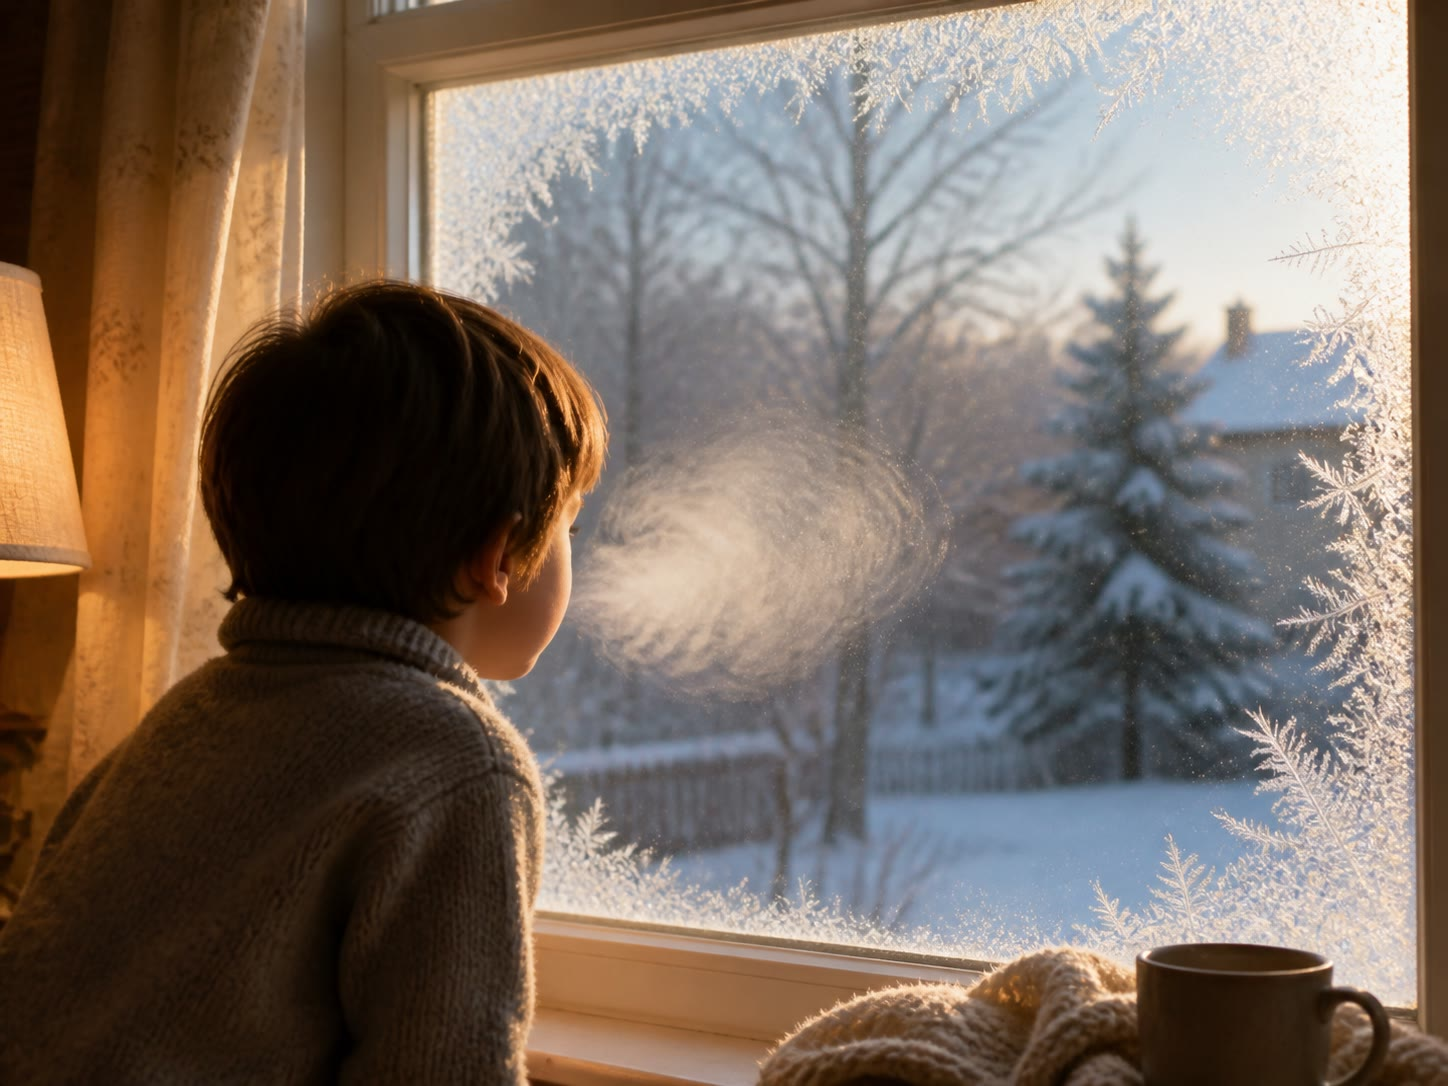
\includegraphics[width=0.56\linewidth]{images/book1/ai/g4-breathing-mist.jpg}

{\small Udara yang diembuskan dibuat terlihat: hangat, lembap --- dan
tanpa terlihat lebih miskin oksigen, lebih kaya karbon dioksida.}
\end{omfigure}

\begin{method}[Merawat napas]\label{met:g4:breathing:care}
\begin{enumerate}
  \item Anginkan ruangan setiap hari --- banyak orang bernapas di
        ruangan tertutup berarti udara yang pengap dan kaya karbon
        dioksida;
  \item bernapaslah lewat hidung di udara yang dingin atau berdebu:
        hidung menghangatkan, melembapkan dan menyaring;
  \item berlarilah, berenanglah, bermainlah --- \omterm{def:g4:breathing:organs}{paru-paru} dan \omterm{def:g3:bones-and-muscles:muscle}{otot}
        \omterm{def:g4:breathing:movements}{pernapasan} yang dilatih tumbuh lebih kuat dan lebih dalam;
  \item jauhkan asap dari paru-parumu: asap mengotori kantongnya yang
        halus, dan kantong itu membersihkan dirinya hanya dengan
        lambat.
\end{enumerate}
\end{method}

\section{Latihan}

\begin{exercise}[$\star$]\label{exo:g4:breathing:1}
Sebutkan kedua gerakan bernapas dan apa yang dilakukan dada pada tiap
gerakannya.
\end{exercise}

\begin{exercise}[$\star$]\label{exo:g4:breathing:2}
Telusurilah jalan satu tarikan napas dari hidung sampai ke kantong
udara yang mungil.
\end{exercise}

\begin{exercise}[$\star$]\label{exo:g4:breathing:3}
Kira-kira berapa kali semenit seorang anak yang tenang dan sedang
beristirahat bernapas? Apa yang terjadi pada bilangan itu ketika
berlari cepat, dan mengapa?
\end{exercise}

\begin{exercise}[$\star$]\label{exo:g4:breathing:4}
Gas mana yang diambil tubuh dari udara, dan gas mana yang
dikembalikannya? Di mana tepatnya pertukaran itu terjadi?
\end{exercise}

\begin{exercise}[$\star$]\label{exo:g4:breathing:5}
Bagaimana udara yang diembuskan berbeda dari udara yang ditarik masuk?
Sebutkan tiga perbedaan.
\end{exercise}

\begin{exercise}[$\star$]\label{exo:g4:breathing:6}
Mengapa \omterm{def:g4:breathing:organs}{paru-paru} dibangun sebagai jutaan kantong mungil alih-alih dua
kantung sederhana? Organ mana lagi pada tahun ini yang memakai kiat
yang sama?
\end{exercise}

\begin{exercise}[$\star$]\label{exo:g4:breathing:7}
Mengapa lebih baik bernapas lewat hidung pada hari yang membekukan
atau berdebu?
\end{exercise}

\begin{exercise}[$\star$]\label{exo:g4:breathing:8}
Cobalah: sambil duduk tenang, hitunglah tarikan napasmu selama satu
menit. Lalu lakukan dua puluh lompatan bintang dan hitunglah lagi.
Laporkan kedua bilangannya lalu jelaskan perubahannya.
\end{exercise}

\begin{exercise}[$\star\star$]\label{exo:g4:breathing:9}
Santapan dapat menunggu berjam-jam; bernapas tidak dapat menunggu satu
menit. Apa yang dikatakannya tentang seberapa banyak oksigen yang
disimpan tubuh, dibandingkan dengan \omterm{def:g3:animals-through-seasons:active}{cadangan makanannya}?
\end{exercise}

\begin{exercise}[$\star\star$]\label{exo:g4:breathing:10}
Sebuah ruang kelas terasa ``pengap'' menjelang siang. Apa yang berubah
pada udaranya, menurut \cref{prop:g4:breathing:exchange}, dan apa yang
diresepkan \cref{met:g4:breathing:care}?
\end{exercise}

\begin{exercise}[$\star\star\star$]\label{exo:g4:breathing:11}
\omterm{prop:g3:sorting-living-things:groups}{Ikan} trout tidak punya \omterm{def:g4:breathing:organs}{paru-paru}: air mengalir melewati insangnya yang
berumbai, dan oksigen yang \emph{terlarut di dalam air} menyeberang ke
dalam \omterm{prop:g4:journey-of-food:absorb}{darahnya} di situ. Tugas apa yang dibagi bersama oleh insang dan
\omterm{def:g4:breathing:organs}{paru-paru}? Dan mengapa seekor \omterm{prop:g3:sorting-living-things:groups}{ikan} trout tercekik di udara, tempat
oksigen berlimpah? (Petunjuk: di luar air, permukaan insang yang
berumbai itu ambruk lalu saling melekat.)
\end{exercise}
